\documentclass{beamer}
\usepackage[UKenglish]{babel}
\usepackage[UKenglish]{isodate}
\usepackage{graphicx}
\usepackage{subcaption}
\usepackage{tikz}
\usepackage{adjustbox}
\usetikzlibrary{arrows}

\author{Paulius Dilkas}
\title{Clique-Based Encodings for Graph Edit Distance}
\date{5th September 2017}

\begin{document}
\maketitle
\begin{frame}{The problem}
  \begin{figure}
    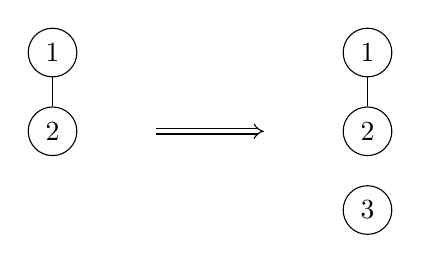
\begin{tikzpicture}
      \begin{scope}[every node/.style={circle,draw}]
        \node (a1) {1};
        \node (a2) [below of=a1] {2};
      \end{scope}
      \path (a1) edge node {} (a2);
      \begin{scope}[every node/.style={circle,draw},xshift=4 cm]
        \node (b1) {1};
        \node (b2) [below of=b1] {2};
        \node (b3) [below of=b2] {3};
      \end{scope}
      \path (b1) edge node {} (b2);
      \draw[-implies,double equal sign distance,shorten >=1cm,shorten <=1cm] (a2) -- (b2);
    \end{tikzpicture}
  \end{figure}
%  \begin{figure}
%    \begin{subfigure}[t]{0.25\textwidth}
%      \vskip 0pt
%      \centering
%      \begin{tikzpicture}
%        \begin{scope}[every node/.style={circle,draw}]
%          \node (a1) {1};
%          \node (a2) [below of=a1] {2};
%        \end{scope}
%        \path (a1) edge node {} (a2);
%      \end{tikzpicture}
%    \end{subfigure}
%    \begin{subfigure}[t]{0.25\textwidth}
%      \vskip 0pt
%      \centering
%      \begin{tikzpicture}
%        \begin{scope}[every node/.style={circle,draw},xshift=4 cm]
%          \node (b1) {1};
%          \node (b2) [below of=b1] {2};
%          \node (b3) [below of=b2] {3};
%        \end{scope}
%        \path (b1) edge node {} (b2);
%      \end{tikzpicture}
%    \end{subfigure}
%  \end{figure}
\end{frame}
\begin{frame}
  \begin{adjustbox}{max totalsize={0.9\textwidth}{0.9\textheight},center}
    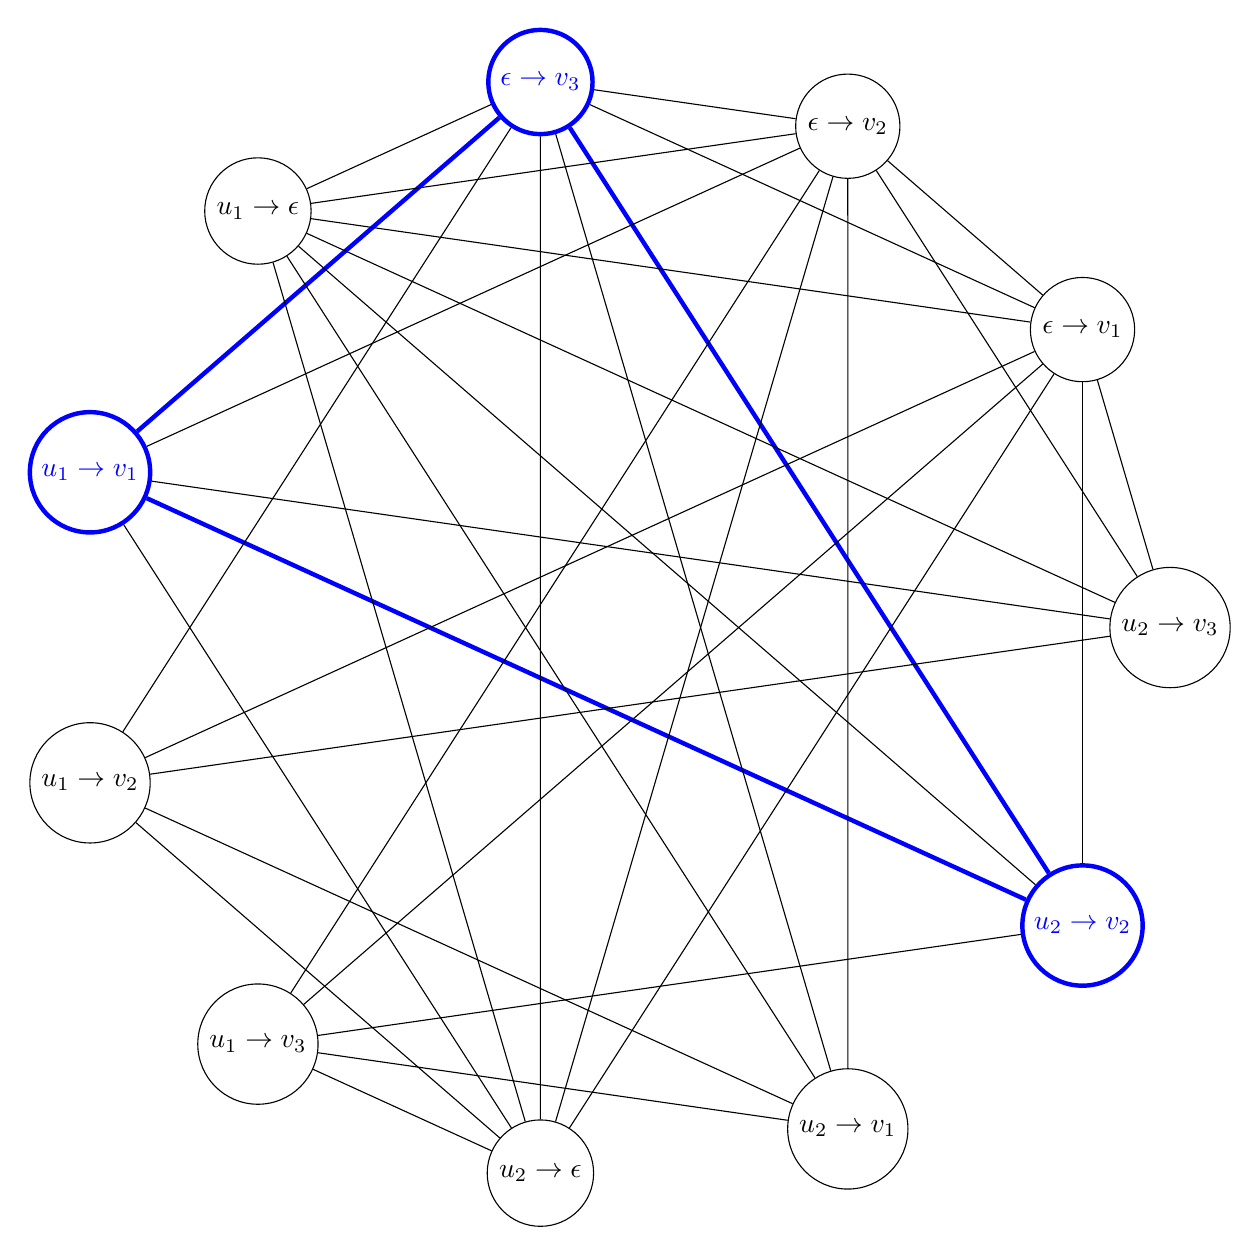
\begin{tikzpicture}
      \begin{scope}[every node/.style={circle,draw}]
        \node (i1) at (360/11 * 1:7cm) {$\epsilon \to v_1$};
        \node (i2) at (360/11 * 2:7cm) {$\epsilon \to v_2$};
        \node (i3) [color=blue,ultra thick] at (360/11 * 3:7cm) {$\epsilon \to v_3$};

        \node (d1) at (360/11 * 4:7cm) {$u_1 \to \epsilon$};
        \node (s11) [color=blue,ultra thick] at (360/11 * 5:7cm) {$u_1 \to v_1$};
        \node (s12) at (360/11 * 6:7cm) {$u_1 \to v_2$};
        \node (s13) at (360/11 * 7:7cm) {$u_1 \to v_3$};

        \node (d2) at (360/11 * 8:7cm) {$u_2 \to \epsilon$};
        \node (s21) at (360/11 * 9:7cm) {$u_2 \to v_1$};
        \node (s22) [color=blue,ultra thick] at (360/11 * 10:7cm) {$u_2 \to v_2$};
        \node (s23) at (360:7cm) {$u_2 \to v_3$};
      \end{scope}

      \begin{scope}[color=blue]
        \path (s11) [ultra thick] edge node {} (s22) edge node {} (i3);
        \path (s22) [ultra thick] edge node {} (i3);
      \end{scope}

      \path (i1) edge node {} (i2) edge node {} (i3) edge node {} (d1) edge node {} (s12) edge node {} (s13) edge node {} (d2) edge node {} (s22) edge node {} (s23);
      \path (i2) edge node {} (i3) edge node {} (d1) edge node {} (s11) edge node {} (s13) edge node {} (d2) edge node {} (s21) edge node {} (s23);
      \path (i3) edge node {} (d1) edge node {} (s12) edge node {} (d2) edge node {} (s21);
      \path (d1) edge node {} (d2) edge node {} (s21) edge node {} (s22) edge node {} (s23);
      \path (s11) edge node {} (d2) edge node {} (s23);
      \path (s12) edge node {} (d2) edge node {} (s21) edge node {} (s23);
      \path (s13) edge node {} (d2) edge node {} (s21) edge node {} (s22);
    \end{tikzpicture}
  \end{adjustbox}
\end{frame}
\begin{frame}
  \begin{adjustbox}{max totalsize={0.9\textwidth}{0.9\textheight},center}
    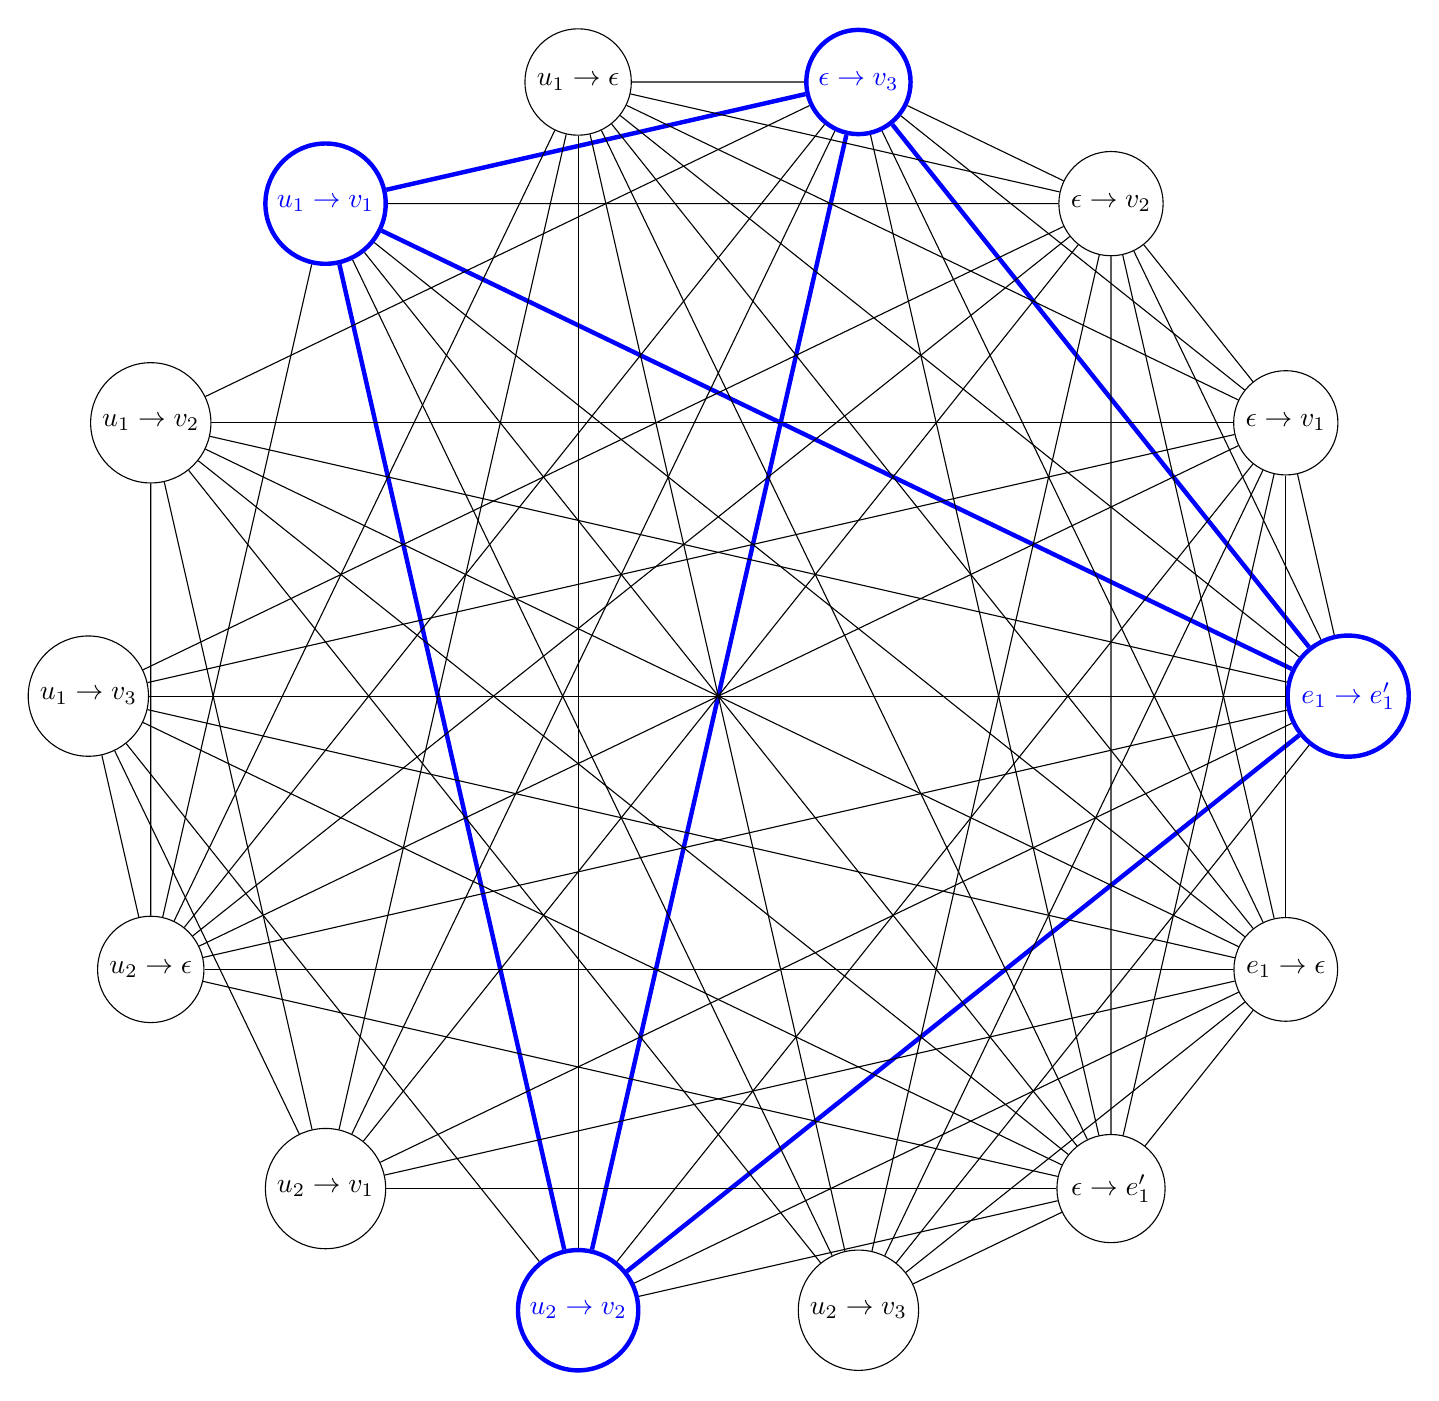
\begin{tikzpicture}
      \begin{scope}[every node/.style={circle,draw}]
        \node (vi1) at (360/14 * 1:8cm) {$\epsilon \to v_1$};
        \node (vi2) at (360/14 * 2:8cm) {$\epsilon \to v_2$};
        \node (vi3) [color=blue,ultra thick] at (360/14 * 3:8cm) {$\epsilon \to v_3$};

        \node (vd1) at (720/7:8cm) {$u_1 \to \epsilon$};
        \node (vs11) [color=blue,ultra thick] at ({720/7 + 360/14 * 1}:8cm) {$u_1 \to v_1$};
        \node (vs12) at ({720/7 + 360/14 * 2}:8cm) {$u_1 \to v_2$};
        \node (vs13) at ({720/7 + 360/14 * 3}:8cm) {$u_1 \to v_3$};

        \node (vd2) at (720/7 + 360/14 * 4:8cm) {$u_2 \to \epsilon$};
        \node (vs21) at ({720/7 + 360/14 * 4 + 360/14 * 1}:8cm) {$u_2 \to v_1$};
        \node (vs22) [color=blue,ultra thick] at ({720/7 + 360/14 * 4 + 360/14 * 2}:8cm) {$u_2 \to v_2$};
        \node (vs23) at ({720/7 + 360/14 * 4 + 360/14 * 3}:8cm) {$u_2 \to v_3$};

        \node (ei) at (2160/7:8cm) {$\epsilon \to e_1'$};
        \node (ed) at (2340/7:8cm) {$e_1 \to \epsilon$};
        \node (es) [color=blue,ultra thick] at (360:8cm) {$e_1 \to e_1'$};
      \end{scope}

      \begin{scope}[draw=blue]
        \path (vi3) [ultra thick] edge node {} (vs11) edge node {} (vs22) edge node {} (es);
        \path (vs11) [ultra thick] edge node {} (vs22) edge node {} (es);
        \path (vs22) [ultra thick] edge node {} (es);
      \end{scope}

      \path (vi1) edge node {} (vi2) edge node {} (vi3) edge node {} (vd1) edge node {} (vs12) edge node {} (vs13) edge node {} (vd2) edge node {} (vs22) edge node {} (vs23) edge node {} (ei) edge node {} (ed) edge node {} (es);
      \path (vi2) edge node {} (vi3) edge node {} (vd1) edge node {} (vs11) edge node {} (vs13) edge node {} (vd2) edge node {} (vs21) edge node {} (vs23) edge node {} (ei) edge node {} (ed) edge node {} (es);
      \path (vi3) edge node {} (vd1) edge node {} (vs12) edge node {} (vd2) edge node {} (vs21) edge node {} (ei) edge node {} (ed);
      \path (vd1) edge node {} (vd2) edge node {} (vs21) edge node {} (vs22) edge node {} (vs23) edge node {} (ei) edge node {} (ed) edge node {} (es);
      \path (vs11) edge node {} (vd2) edge node {} (vs23) edge node {} (ei) edge node {} (ed);
      \path (vs12) edge node {} (vd2) edge node {} (vs21) edge node {} (vs23) edge node {} (ei) edge node {} (ed) edge node {} (es);
      \path (vs13) edge node {} (vd2) edge node {} (vs21) edge node {} (vs22) edge node {} (ei) edge node {} (ed) edge node {} (es);
      \path (vd2) edge node {} (ei) edge node {} (ed) edge node {} (es);
      \path (vs21) edge node {} (ei) edge node {} (ed) edge node {} (es);
      \path (vs22) edge node {} (ei) edge node {} (ed);
      \path (vs23) edge node {} (ei) edge node {} (ed) edge node {} (es);
      \path (ei) edge node {} (ed);
    \end{tikzpicture}
  \end{adjustbox}
\end{frame}
\begin{frame}
  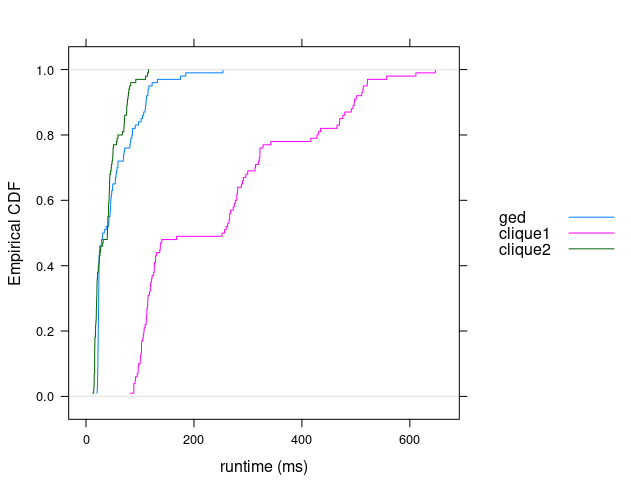
\includegraphics[scale=0.6]{../comparison.png}
\end{frame}
\begin{frame}
  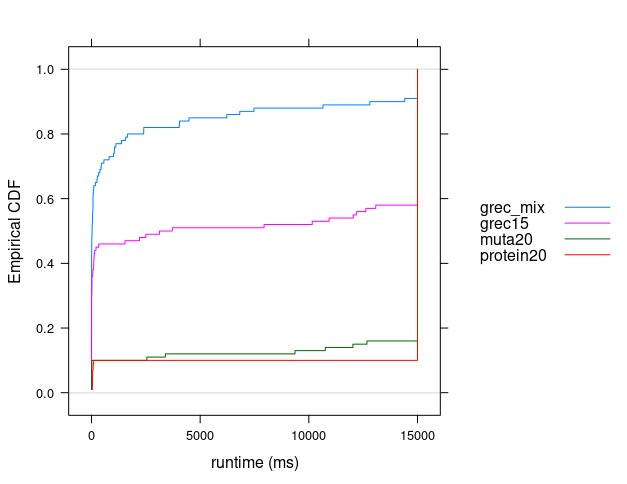
\includegraphics[scale=0.6]{../ecdfs.png}
\end{frame}
\end{document}
